\documentclass{article}

\usepackage{tikz}
\usetikzlibrary{shapes.geometric}

\setlength{\parindent}{0in}

\newcommand{\splitpage}{\vfill\hrule\vfill}

\begin{document}
%\Large

You have been given $\fbox{$4 + 1$}$ numbers,
$$
a, \quad b, \quad c, \quad d, \quad, e
$$
and you would like to compute $abcde$.  You can only multiply two numbers at a time, so you could compute
$abcde$ by computing $(a((bc)d))e$.  How many different ways can you
perform this calculation?

%\pagebreak\null\pagebreak
\splitpage

There are $\fbox{$2 \times 4$}$ people seated around a table.  How many ways can
they all be simultaneously shaking hands with another person at the
table so that none of the arms cross each other?

\begin{center}
\begin{tikzpicture}
% create the node
\node[draw=none,minimum size=3cm,regular polygon,regular polygon sides=8] (a) {};

% draw a black dot in each vertex
\foreach \x in {1,2,...,8}
  \fill (a.corner \x) circle[radius=2pt];

\draw (a.corner 1) -- (a.corner 2);
\draw (a.corner 3) -- (a.corner 4);
\draw (a.corner 5) -- (a.corner 6);
\draw (a.corner 7) -- (a.corner 8);

\end{tikzpicture}
\quad\raisebox{1.5cm}{or}\quad
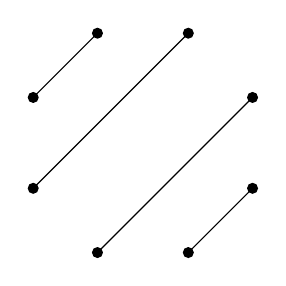
\begin{tikzpicture}
% create the node
\node[draw=none,minimum size=3cm,regular polygon,regular polygon sides=8] (a) {};

% draw a black dot in each vertex
\foreach \x in {1,2,...,8}
  \fill (a.corner \x) circle[radius=2pt];

\draw (a.corner 1) -- (a.corner 4);
\draw (a.corner 2) -- (a.corner 3);
\draw (a.corner 5) -- (a.corner 8);
\draw (a.corner 6) -- (a.corner 7);

\end{tikzpicture}
\quad\raisebox{1.5cm}{or \ldots?}
\end{center}

%\pagebreak\null\pagebreak
\splitpage

A $\fbox{$4 + 2$}$-sided regular polygon can be divided into four triangles.
In how many different ways can this be done?

\begin{center}
\begin{tikzpicture}
% create the node
\node[draw=none,minimum size=3cm,regular polygon,regular polygon sides=6] (a) {};

% draw a black dot in each vertex
\foreach \x in {1,2,...,6}
  \fill (a.corner \x) circle[radius=2pt];
\foreach \x [evaluate = \y as \y using int(\x+1)] in {1,2,...,6}
  \draw (a.corner \x) -- (a.corner \y);

\draw (a.corner 1) -- (a.corner 3);
\draw (a.corner 1) -- (a.corner 4);
\draw (a.corner 1) -- (a.corner 5);

\end{tikzpicture}
\quad\raisebox{1.5cm}{or}\quad
\begin{tikzpicture}
% create the node
\node[draw=none,minimum size=3cm,regular polygon,regular polygon sides=6] (a) {};

% draw a black dot in each vertex
\foreach \x in {1,2,...,6}
  \fill (a.corner \x) circle[radius=2pt];
\foreach \x [evaluate = \y as \y using int(\x+1)] in {1,2,...,6}
  \draw (a.corner \x) -- (a.corner \y);

\draw (a.corner 1) -- (a.corner 3);
\draw (a.corner 3) -- (a.corner 5);
\draw (a.corner 1) -- (a.corner 5);
%\draw (a.corner 1) -- (a.corner 5);

\end{tikzpicture}
\quad\raisebox{1.5cm}{or \ldots?}
\end{center}

\pagebreak
%\splitpage

How many mountain ranges can you build with $\fbox{$4$}$ uphill and downhill strokes?

\newcommand*{\xMin}{0}%
\newcommand*{\xMax}{8}%
\newcommand*{\yMin}{0}%
\newcommand*{\yMax}{4}%
\begin{center}
\begin{tikzpicture}[x=0.5cm,y=0.5cm]
    \foreach \i in {\xMin,...,\xMax} {
        \draw [very thin,gray] (\i,\yMin) -- (\i,\yMax);%  node [below] at (\i,\yMin) {$\i$};
    }
    \foreach \i in {\yMin,...,\yMax} {
        \draw [very thin,gray] (\xMin,\i) -- (\xMax,\i);% node [left] at (\xMin,\i) {$\i$};
    }

\draw[thick] (0,0) -- (1,1) -- (2,2) -- (3,1) -- (4,2) -- (5,1) -- (6,0) -- (7,1) -- (8,0);

\end{tikzpicture}
\quad\raisebox{1cm}{or}\quad
\begin{tikzpicture}[x=0.5cm,y=0.5cm]
    \foreach \i in {\xMin,...,\xMax} {
        \draw [very thin,gray] (\i,\yMin) -- (\i,\yMax);%  node [below] at (\i,\yMin) {$\i$};
    }
    \foreach \i in {\yMin,...,\yMax} {
        \draw [very thin,gray] (\xMin,\i) -- (\xMax,\i);% node [left] at (\xMin,\i) {$\i$};
    }

\draw[thick] (0,0) -- (1,1) -- (2,0) -- (3,1) -- (4,2) -- (5,3) -- (6,2) -- (7,1) -- (8,0);

\end{tikzpicture}
\quad\raisebox{1cm}{or\ldots?}
\end{center}

%\pagebreak\null\pagebreak
\splitpage

Let $n = \fbox{$4$}$.  In an $n \times n$ grid of squares, how many
paths are there of length $2n$ that lead from the upper-left corner to
the bottom-right corner without touching the thick diagonal line?

\renewcommand*{\xMin}{0}%
\renewcommand*{\xMax}{4}%
\renewcommand*{\yMin}{0}%
\renewcommand*{\yMax}{4}%
\begin{center}
\begin{tikzpicture}
    \foreach \i in {\xMin,...,\xMax} {
        \draw [very thin,gray] (\i,\yMin) -- (\i,\yMax);%  node [below] at (\i,\yMin) {$\i$};
    }
    \foreach \i in {\yMin,...,\yMax} {
        \draw [very thin,gray] (\xMin,\i) -- (\xMax,\i);% node [left] at (\xMin,\i) {$\i$};
    }

\draw[very thick] (-.1,3.9) -- (3.9,-0.1);

\draw[thick] (0,4) -- (1,4) -- (2,4) -- (2,3) -- (3,3) -- (4,3) -- (4,2) -- (4,1) -- (4,0);

%\draw [step=1.0,blue, very thick] (0,0)  (5.5,4.5);
%\draw [very thick, brown, step=1.0cm,xshift=-0.5cm, yshift=-0.5cm] (0.5,0.5) grid +(5.5,4.5);
\end{tikzpicture}
\quad\raisebox{2cm}{or}\quad
\begin{tikzpicture}
    \foreach \i in {\xMin,...,\xMax} {
        \draw [very thin,gray] (\i,\yMin) -- (\i,\yMax);%  node [below] at (\i,\yMin) {$\i$};
    }
    \foreach \i in {\yMin,...,\yMax} {
        \draw [very thin,gray] (\xMin,\i) -- (\xMax,\i);% node [left] at (\xMin,\i) {$\i$};
    }

\draw[very thick] (-.1,3.9) -- (3.9,-0.1);

\draw[thick] (0,4) -- (1,4) -- (1,3) -- (2,3) -- (3,3) -- (3,2) -- (3,1) -- (4,1) -- (4,0);

%\draw [step=1.0,blue, very thick] (0,0)  (5.5,4.5);
%\draw [very thick, brown, step=1.0cm,xshift=-0.5cm, yshift=-0.5cm] (0.5,0.5) grid +(5.5,4.5);
\end{tikzpicture}
\quad\raisebox{2cm}{or\ldots?}
\end{center}

%\pagebreak\null\pagebreak
\splitpage

Build strings of length $\fbox{$2 \times 4$}$ with $\fbox{$4$}$ \textsf{X}s and
$\fbox{$4$}$ \textsf{O}s with the following property: no initial segment has
more \textsf{O}s than \textsf{X}s.  The strings \textsf{XXXOOOXO} and
\textsf{XOXOXXOO}.  How many such strings are there?

%\pagebreak\null\pagebreak
\splitpage

You have been given $\fbox{$4$}$ pairs of parentheses, i.e., you have
four opening parentheses \textsf{(}s and four closing parentheses
\textsf{)}s.  In how many valid ways can you place them, meaning each
opening parenthesis has a closing parenthesis?  For instance,
\textsf{(())()()} is valid, but \textsf{))(())((} is not valid.



\end{document}
